\chapter{Sviluppo Back-end con GeoServer}
\label{cap:chapter5}

\section{Soluzione al problema}

La prima soluzione ideata dal candidato è stata quella di realizzare un server, proprietario dell'azienda, in cui scaricare al suo interno tutte le mappe interessate. L'idea prevedeva la realizzazione di un programma in grado di contattare uno ad uno tutti i server WMS esterni, e scaricare all'interno del server aziendale tutte le mappe disponibili, rispettando ovviamente eventuali rate-limiting imposti. In questo modo, si sarebbero evitati potenziali problemi legati alla latenza dei server e alla possibilità che un servizio diventasse improvvisamente non disponibile.
\\Il problema in questo tipo di implementazione è che il peso delle mappe è estremamente elevato, rendendo quindi molto dispendioso, sia in termini di risorse di calcolo che economiche, realizzare una piattaforma di questo genere. 
\\Innanzitutto, va considerato che non tutte le mappe WMS sono ospitate sugli stessi server; alcuni di essi potrebbero offrire prestazioni migliori e addirittura non applicare alcun tipo di limitazione sulla frequenza delle richieste. In aggiunta, non tutte le mappe richieste dall'applicazione hanno la stessa importanza: potrebbe accadere che alcune mappe vengano frequentemente consultate dagli utenti, mentre altre siano utilizzate raramente, causando un consumo inutile di spazio e risorse. 
\\Inoltre, è importante anche considerare che i server WMS potrebbero aggiungere dei nuovi layer alla richiesta di GetCapabilities in futuro; questo richiederebbe non solo la creazione di un meccanismo per copiare tutte le mappe, ma anche di mantenerle sincronizzate costantemente. Oppure, se in futuro si dovesse aggiungere un nuovo servizio all'interno del programma, risulterebbe laborioso aggiungere manualmente un nuovo server da cui reperire le mappe desiderate, tenendo in considerazione che non tutti i server potrebbero offrire le mappe nello stesso modo. Infatti, come già mostrato, OpenLayers utilizza il campo \verb|serverType| per cambiare il modo in cui esegue le richieste sui vari server di mappe.
\\Infine, poiché la piattaforma è destinata alla commercializzazione, è essenziale considerare l'origine delle mappe: non tutte le mappe sono disponibili con termini di utilizzo che consentono di poterle scaricare e usare gratuitamente a fini commerciali. Alcune richiedono un contatto diretto con i loro server e non offrono legalmente la possibilità di poter scaricare le mappe.
\\Questo non esclude la possibilità che questo tipo di implementazione possa essere sviluppata in futuro, magari limitandola solo alle mappe di maggiore importanza o a quelle che frequentemente presentano problematiche di funzionamento, rendendole quindi inutilizzabili.
\\~\\
Una soluzione più semplice da adottare consisterebbe nell'implementare un meccanismo che si occupi di fare "proxying" dei server esterni, cioè ogniqualvolta che il front-end richiede una mappa, anziché contattare direttamente il server WMS interessato, l'applicazione potrebbe contattare un nostro servizio intermedio. Quest'ultimo, a sua volta, inoltrerebbe la richiesta al server WMS esterno e restituirebbe la risposta al front-end. 
\\Attraverso un meccanismo di questo tipo, sarebbe possibile implementare un sistema di caching delle risposte ottenute dai server WMS esterni: quando il nostro servizio intermedio riceve una richiesta di mappa dal front-end, può verificare se questa è già presente nella cache. Se lo è e non è stata invalidata, il servizio può restituirla  senza dover contattare nuovamente il server esterno.
\\Inoltre, se il programma fosse eseguito all'interno di un WebServer, si avrebbe l'opportunità di sfruttare ulteriori meccanismi di caching: il WebServer potrebbe essere configurato per memorizzare nella sua cache le risposte alle richieste già effettuate al servizio intermedio. Ciò significa che se il client contattasse il WebServer per ricevere una mappa, questo potrebbe direttamente restituirla senza comunicare con il sistema precedentemente citato.
\\Un meccanismo di questo tipo, inoltre, adotterebbe un approccio centralizzato, permettendo ai client di interagire esclusivamente con un unico servizio, semplificando così anche il processo di gestione delle richieste. In questo modo, il modello potrebbe essere esteso per includere anche altri protocolli, come ad esempio il WFS.
\\Questa soluzione non solo affronterebbe il problema del rate-limiting e della lentezza dei server esterni, ma risolverebbe anche le preoccupazioni legate ai termini di utilizzo delle mappe spiegati precedentemente.
\\In conclusione, tale implementazione potrebbe anche essere estesa, andando a realizzare un sistema che permetta di sfruttare altri protocolli più efficienti rispetto allo standard WMS. Ad esempio, si potrebbe realizzare un sistema che, dopo aver ricevuto la risposta dal server WMS esterno, potrebbe convertire l'immagine suddividendola in tiles, per poi restituirle al client tramite protocollo WMTS. Tale meccanismo, già realizzato da altri, prende il nome di GeoServer.

\section{Introduzione a GeoServer}

GeoServer è un software OpenSource scritto in Java che permette di caricare e servire dati di mappe geospaziali.
All'interno di questo programma i dati possono essere caricati in vari formati (come Shapefile, GeoPackage, etc...) per poi essere esposti attraverso l'utilizzo di protocolli standard OGC (come WMS, WMTS, WFS, etc...), oppure attraverso l'utilizzo di altri protocolli come TMS.
Ad esempio, è possibile caricare un file di mappa in formato Shapefile ed esporlo sul proprio server mediante un servizio WMS.
In questo modo un client che supporta tale protocollo, come appunto OpenLayers, può visualizzare la mappa interessata e richiederla in un formato raster come PNG, JPG o simili.

\subsection{Caratteristiche principali}

Come già accennato, una delle funzionalità principali del GeoServer è il "proxying" di servizi OGC, ovvero consente di replicare e mantenere aggiornati i servizi di mappe forniti da server esterni.
\\Ciò è possibile in quanto il GeoServer è in grado di memorizzare al suo interno l'URL che rappresenta la richiesta di GetCapabilities. Come già spiegato, questa richiesta è essenziale per ottenere tutte le informazioni necessarie (layer di mappe, proiezioni, formati, etc...) al fine di richiedere le mappe fornite dal server esterno.
\\In pratica, ogni volta che un client richiede al GeoServer una mappa che non è presente localmente, il GeoServer inizia contattando il server esterno tramite una richiesta di GetCapabilities. Una volta ricevuta la risposta, il GeoServer esegue un'altra richiesta (ad esempio una GetMap nel caso dei servizi WMS) per ottenere la mappa specifica richiesta dal client. Una volta che il GeoServer riceve i dati della mappa dal server esterno, li invia al client come risposta alla sua richiesta originale.
\\Questo consente di memorizzare tutti i dati delle mappe, potenzialmente anche esposte medianti protocolli diversi, sotto un unico server. Tale pratica non solo semplifica la gestione e la manutenzione dei dati geospaziali, ma dal punto di vista del client, viene offerta l'illusione di avere un sistema centralizzato, in cui tutte le mappe sono contenute direttamente sotto un unico servizio.
\\Un'altra importante funzionalità di GeoServer è la capacità di esporre dati geospaziali utilizzando protocolli diversi. 
Ad esempio, è possibile registrare un server esterno di mappe WMS nel modo spiegato precedentemente e successivamente, attraverso GeoServer, renderlo disponibile al client nei protocolli WMS, WMTS, TMS, etc... Questo perché, dal punto di vista del client, la comunicazione avviene col GeoServer, che maschera qualsiasi eventuale ulteriore comunicazione con server esterni. In questo caso, GeoServer si occuperà in automatico di fornire i dati della mappa in tiles, nonostante il servizio esterno non supportasse tale protocollo.

\subsection{Meccanismi di Caching}

Avere tutte le mappe centralizzate sotto un unico server favorisce anche l'utilizzo di meccanismi di caching: a livello di WebServer, per esempio, tramite l'utilizzo di un Reverse Proxy, è possibile configurare politiche di caching per memorizzare temporaneamente le risposte alle richieste HTTP inviate al GeoServer. Questo consente di ridurre il carico su di esso, in quanto alcune richieste possono essere soddisfatte direttamente dalla cache del WebServer senza doverle inoltrare nuovamente al GeoServer. Tale pratica risulterebbe più complessa da fare, se le mappe fossero decentralizzate su servizi esterni, specialmente se di terze parti.
\\Inoltre, GeoServer stesso offre diversi livelli di caching. È possibile infatti configurarlo per memorizzare in una sua cache interna le risposte alle richieste di mappe.
\\Esiste anche la possibilità di memorizzare nella cache la risposta ottenuta dalla richiesta GetCapabilities inviata ai servizi OGC esterni, in modo da evitarne il recupero ogni volta. Questo risulta utile soprattutto quando si ha a che fare con mappe geospaziali che cambiano raramente nel tempo o che non cambiano affatto, anche se è possibile comunque risolvere il problema in parte mettendo una cache di durata più breve. Questo consente a GeoServer di rispondere più rapidamente alle richieste di mappe, utilizzando i dati già memorizzati nella cache anziché elaborarli nuovamente, riducendo così il carico e migliorando i tempi di risposta.

\subsection{Funzionamento di GeoServer}

Geoserver supporta diversi tipi formati e servizi geospaziali, i più noti sono:

\begin{itemize}
      \item Servizi di mappe: WMS, WMTS, WFS, TMS per i servizi di mappe;
      \item Dati raster: GeoPackage, ArcGrid, GeoTIFF, ImageMosaic, WorldImage;
      \item Dati vettoriali o a oggetti geospaziali: ShapeFiles, GeoPackage, PostGIS;
\end{itemize}
Questi ultimi possono essere caricati e gestiti tramite l'utilizzo di un'interfaccia grafica, realizzata sotto forma di un'applicazione web, oppure tramite l'utilizzo di chiamate ad una REST API.
\\Al fine di poter caricare correttamente una mappa all'interno di GeoServer, è necessario creare tre componenti basilari:
\begin{itemize}
      \item Workspace: rappresenta precisamente "l'area di lavoro", cioè il luogo in cui tutte le mappe vengono effettivamente caricate, quest'ultime a sua volta vengono organizzate in all'interno di Storage. Una workspace può contenere uno o più Storage.
      \item Storage: rappresenta il contenitore di mappe che si vuole caricare all'interno di GeoServer. Può essere un servizio WMS, WMTS, WFS, o un dato geospaziale come Shapefile, GeoTIFF, etc... Ovviamente in base al tipo di Storage che si va a creare, le impostazioni visualizzate sull'interfaccia grafica (o i query params da inviare secondo la REST API) saranno differenti. Per esempio, se si va a creare un servizio esterno WMS, sarà chiesto il link delle capabilities da contattare. Se si andrà a caricare uno Shapefile, sarà richiesto il percorso locale in cui il file si trova.
      \item Layer: rappresenta la mappa effettiva, quella che verrà poi fornita al Front-end. È ciò che restituisce lo storage una volta ricevuta la risposta alla GetCapabilities, nel caso di un servizio OGC, o ciò che contiene uno Shapefile. Ovviamente più layer possono stare all'interno di uno storage.
\end{itemize}
Dal punto di vista di architetturale, come si può vedere dal codice fornito su GitHub [7], GeoServer è stato sviluppato in Java utilizzando Spring come Framework, mentre l’interfaccia grafica è stata realizzata con Wicket. Infine, la REST API è stata anch'essa implementata utilizzando Spring, precisamente con Spring MVC Framework.
\\Una nota importante riguardo la REST API è che, come verrà spiegato più dettagliatamente in seguito, la specifica fornita da GeoServer stesso presenta delle carenze in termini di usabilità e affidabilità: tale specifica, infatti, non è stata più aggiornata con le continue evoluzioni di GeoServer, andando a così a compromettere il suo funzionamento. L'uso delle API di GeoServer è stata una parte integrante del tirocinio e ciò ha complicato notevolmente il suo utilizzo.

\section{Integrazione di GeoServer nel progetto}

Il tirocinio è proseguito con l'installazione del software GeoServer all'interno dell'applicazione. Per garantire una gestione agevole e una configurazione uniforme dell'ambiente di sviluppo, è stato deciso di adottare un'immagine Docker per l'installazione di questo software.
\\Inizialmente, è stata scelta l'immagine Docker ufficiale di GeoServer, fornita direttamente dalla loro pagina GitHub, che è stata installata seguendo il processo di installazione descritto nella loro documentazione.  
Successivamente, poiché tale immagine non supportava l'architettura ARM, la quale era necessaria per esigenze di sviluppo del progetto, è stata adottata una immagine diversa, non ufficiale, presente sempre su GitHub al seguente indirizzo \cite{ImmagineGithubGeoServer}.
\\Per effettuare questa operazione, è stato necessario apportare delle modifiche ai file di configurazione Docker già esistenti nel progetto: inizialmente, è stata aggiunta l'immagine di GeoServer selezionata al file  \verb|compose.yaml| e successivamente, è stato necessario intervenire sul file \verb|compose.override.yaml| per modificare la porta di GeoServer da 8080 a 8888, rendendolo così accessibile, in quanto la porta 8080 era già occupata da un altro servizio.
\\Infine, per rendere disponibile il servizio di GeoServer ad un indirizzo diverso da quello locale (127.0.0.1:8888), è stato configurato il reverse proxy di Caddy in modo da ottenere un dominio con certificazione TLS installata, il quale reindirizzava  direttamente al servizio di GeoServer stesso. 

\subsection{Problematiche riscontrate}

Dopo aver installato con successo l'immagine di Docker, è stato riscontrato un problema relativo alla persistenza dei file generati da GeoServer. Precisamente, all'avvio dell'applicazione all'interno di un container Docker, il GeoServer generava una serie di file in una directory specifica, i quali erano essenziali per il funzionamento dell'applicazione stessa e per mantenere le configurazioni impostate. In aggiunta, ogni volta che venivano caricate delle mappe al suo interno, il GeoServer generava dei file ulteriori per tenere traccia delle mappe appena inserite, anch'essi sempre presenti nello stesso percorso.
% non riesco a dire che quando si modificano delle impostazioni più specifiche si generavano dei nuovi file 
\\Il problema si manifestava quando il container di Docker veniva arrestato, comportando la cancellazione di tutti i dati al suo interno, inclusi i file di configurazione e delle mappe appena menzionati. Di conseguenza, non solo ogni volta che si avviava il container le configurazioni di GeoServer si resettavano, ma le mappe inserite andavano perse.
\\Per risolvere questo problema, è stata implementata una soluzione che utilizza i volumi forniti da Docker stesso, i quali consentono di memorizzare i dati in modo persistente anche dopo la terminazione del container.
\\Infine, per garantire l'accesso alle mappe di GeoCart e di IdroGEO, precedentemente caricate su un drive aziendale di Google, è stato utilizzato Rclone, un software che permette la creazione di cartelle o dischi virtuali collegati ai servizi Cloud. 
\\Precisamente, è stato realizzato uno script in bash che, attraverso l'uso del comando \verb|rclone sync|, scarica automaticamente le mappe dal drive aziendale e le inserisce in una specifica cartella collegata al volume del container di Docker. Grazie a questa configurazione, le mappe venivano così mantenute sincronizzate. La configurazione finale di Docker ottenuta è quindi la seguente:

\begin{lstlisting}[language=Java]{}
  geoserver:
    image: kartoza/geoserver:2.24.2
    environment:
      - GEOSERVER_CSRF_DISABLED=true
      - GEOSERVER_ADMIN_PASSWORD=geoserver
      - GEOSERVER_ADMIN_USER=admin
    restart: unless-stopped
    ports:
      - "8888:8080"
    volumes:
      - ./workspaces/geoserver/scripts/chown-data.sh:/docker-entrypoint-geoserver.d/chown-data.sh
      - ./workspaces/geoserver/data:/opt/geoserver/data_dir
      - ./workspaces/geoserver/layers:/opt/layers
\end{lstlisting}

\section{Integrazione delle mappe con GeoServer}

Il candidato ha proseguito il proprio lavoro studiando il funzionamento di tale software, attraverso la documentazione ufficiale \cite{DocumentazioneGeoServer}. Successivamente, utilizzando l'interfaccia grafica fornita da GeoServer stesso, ha poi iniziato ad interagire con l'applicazione, così da comprendere appieno le funzionalità che offriva. Il tirocinante ha cominciato inserendo alcune mappe all'interno di GeoServer, avviando così una serie di test per valutare la sua operatività e analizzare le prestazioni effettive dell'applicazione.

\subsection{Implementazione protocollo WMS}

\\La prima prova si è concentrata sulle mappe WMS, con l'obbiettivo di valutare il loro comportamento all'interno di GeoServer rispetto alla sua assenza, cercando quindi di comprendere se l'utilizzo di tale software, come server di mappe, influenzasse in qualche modo le prestazioni complessive.
\\Per fare ciò, è stata creata una Workspace al cui interno sono stati inseriti degli Storage. Ognuno di essi, a sua volta, è stato poi configurato per effettuare proxying verso un server WMS esterno. Infine, per ogni Storage, sono stati caricati tutti i layer che vi erano associati, rendendoli così disponibili a trasmettere le immagini di mappa tramite protocollo WMS. Le mappe considerate in questa operazione sono state: la "Carta ecopedologica d’Italia", ovvero la stessa utilizzata precedentemente, in modo da avere un confronto fra le due implementazioni e la carta "Alluvioni - Estensione dell'area allagabile (PGRA 2021)" \ref{fig:italiaAlluvioni}, selezionata per testare una nuova mappa.
\\Il lavoro è poi continuato con la modifica del codice front-end sviluppato in precedenza, cambiando l'indirizzo a cui il client si collegava per recuperare i dati delle mappe. La differenza in questa operazione è stata che, grazie al GeoServer, le mappe potevano essere recuperate attraverso due tipi di richieste GetCapabilities. La prima richiesta, più generale, restituiva la lista di tutti i layer disponibili, indipendentemente dalla Workspace in cui si trovavano. La seconda, invece, conteneva singolarmente la lista di mappe di ogni Workspace, rivelandosi utile per ridurre il peso di ogni richiesta.
\\Per semplificare questa fase di test, è stata scelta la prima opzione nonostante fosse meno efficiente, in quanto è risultato più agevole comprendere se tutti i layer venissero pubblicati correttamente e con le giuste configurazioni.
\\I risultati ottenuti sono stati positivi, riuscendo visualizzare le mappe nello stesso modo in cui erano state mostrate precedentemente. Inoltre, dopo aver abilitato il meccanismo di caching interno a GeoServer per ciascun layer, le prestazioni sono migliorate ulteriormente, riducendo così la necessità di effettuare richieste ai server esterni. Ciò ha portato ad un uso favorevole di GeoServer, considerando così l'opzione di utilizzarlo come server di mappe all'interno del progetto.

\begin{figure}[htbp]
      \centering
      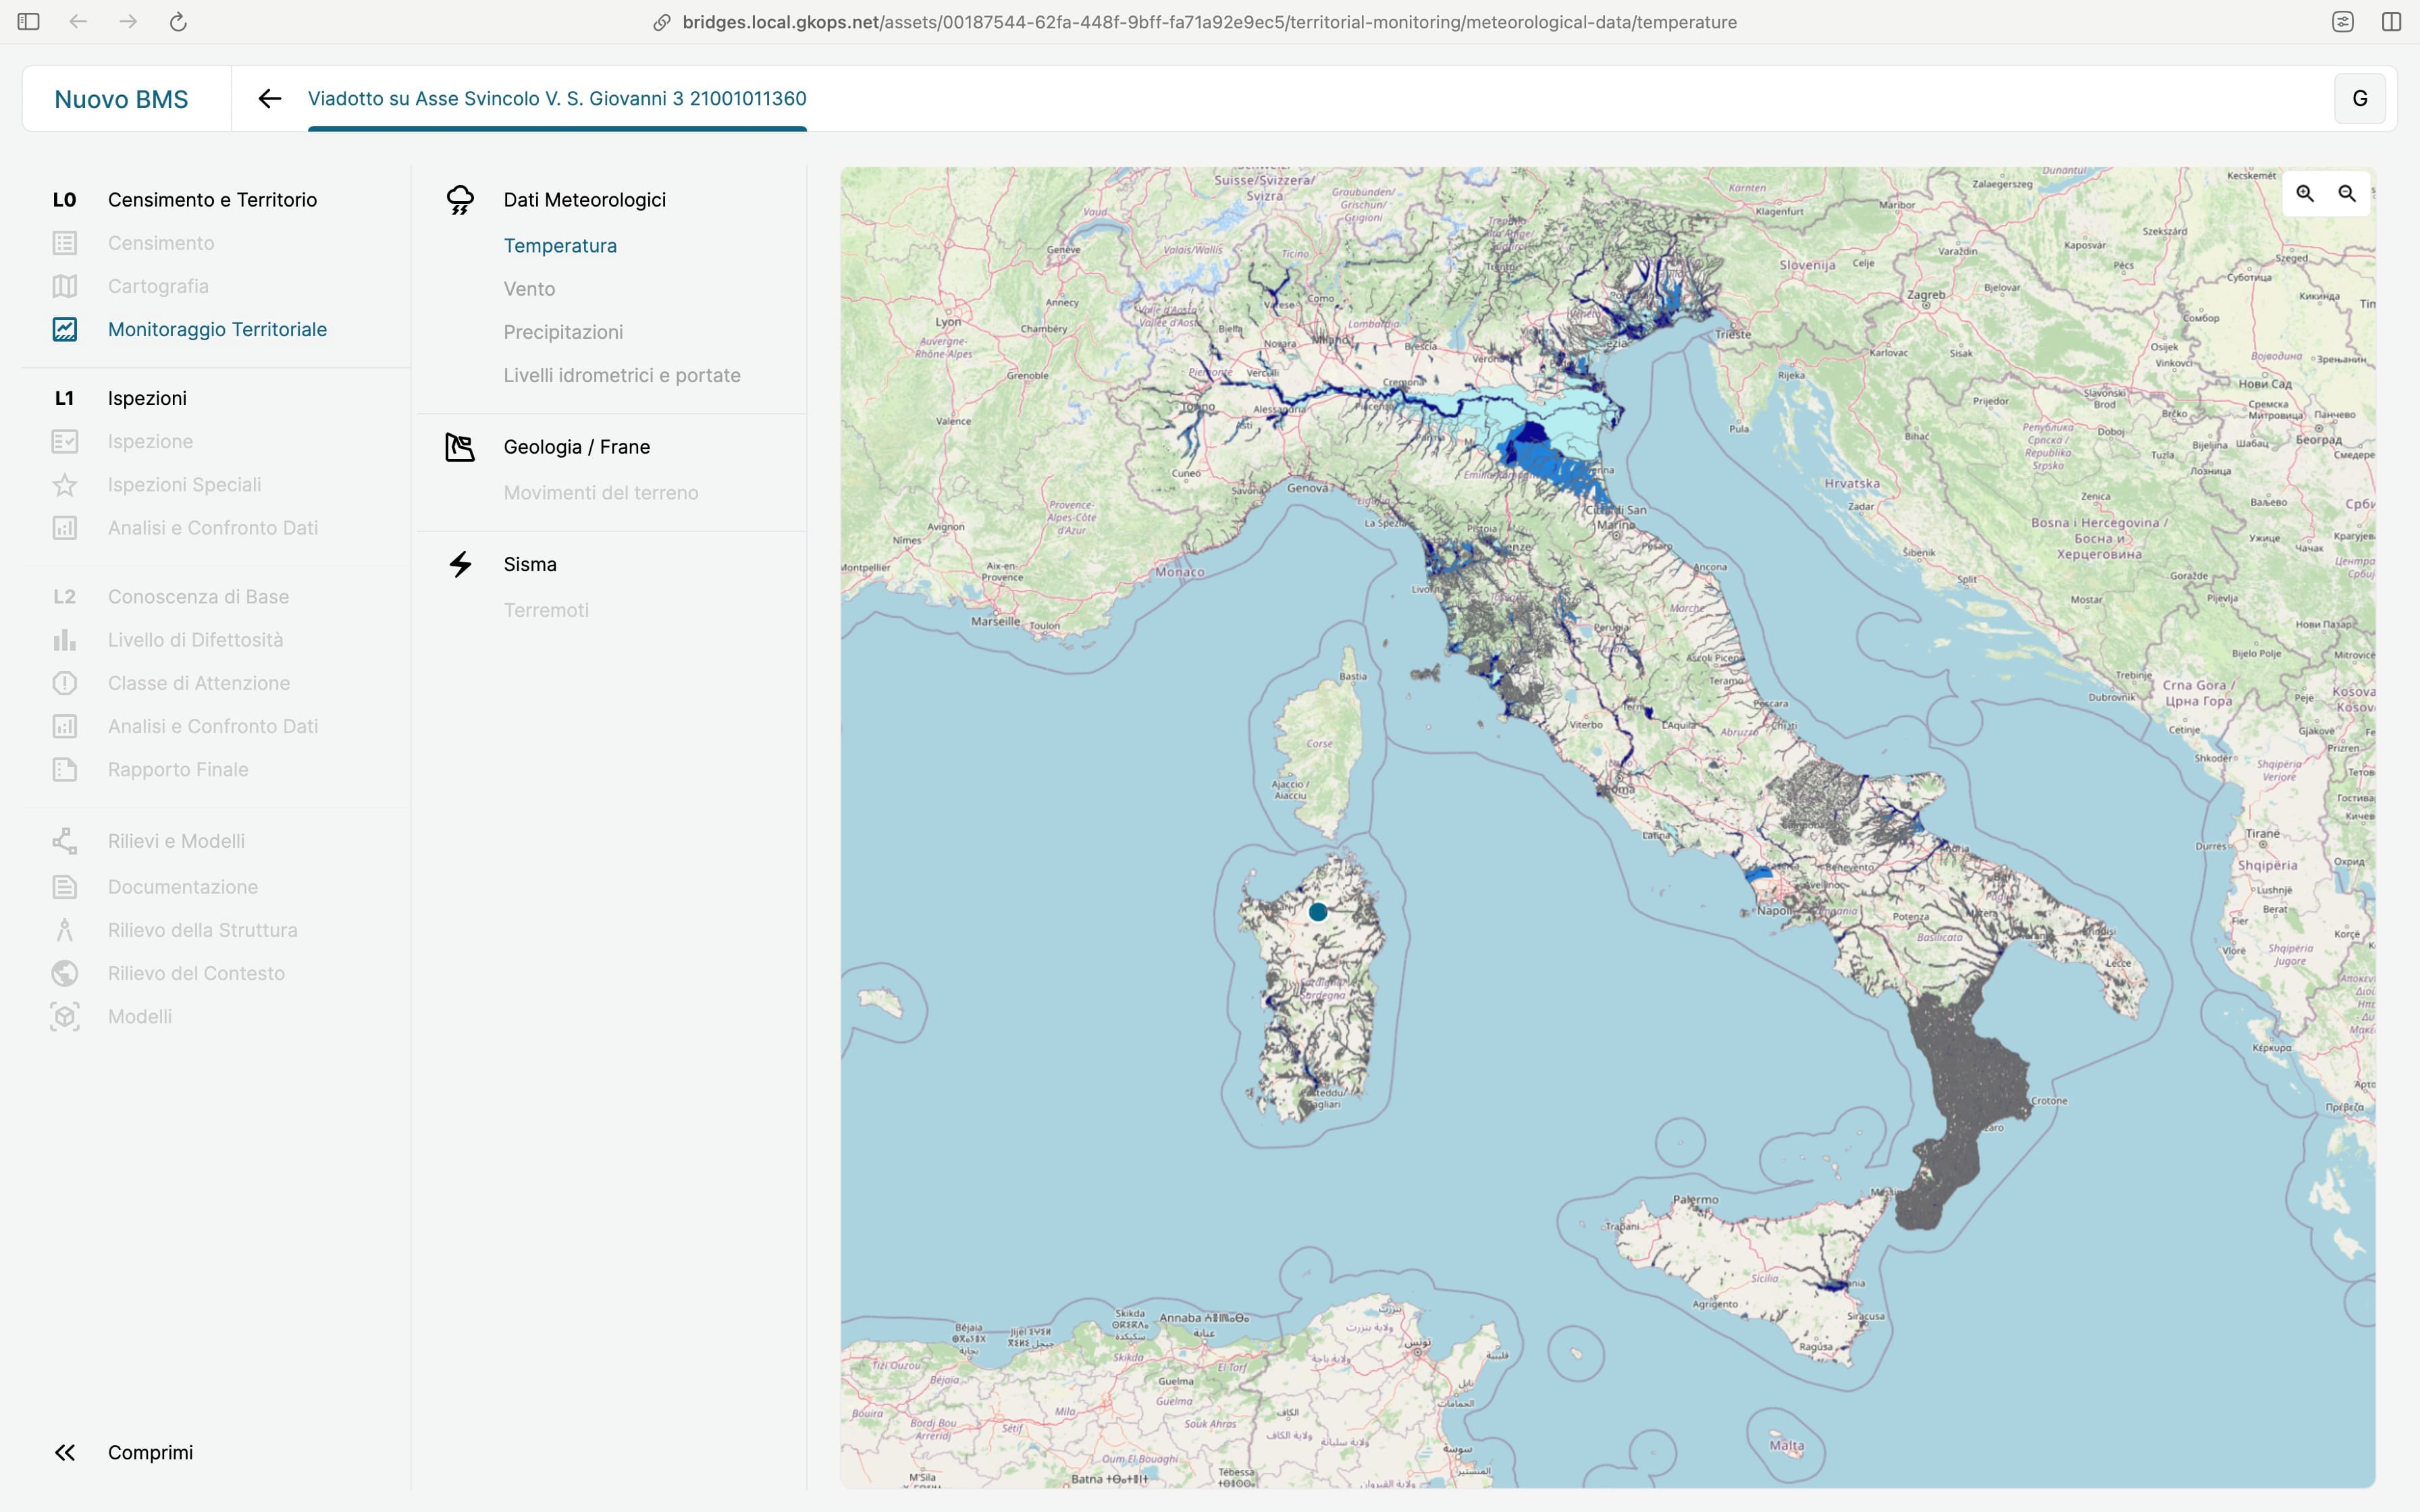
\includegraphics[width=1\textwidth]{Tesi/images/Capitolo5/italiaAlluvioni.jpg}
      \caption{Alluvioni - Estensione dell’area allagabile (PGRA 2021) - WMS}
      \label{fig:italiaAlluvioni}
\end{figure}

\subsection{Implementazione protocollo WMTS}

L'attenzione si è poi rivolta sulla possibilità di utilizzare il protocollo WMTS anziché WMS per servire la stessa mappa, poiché come già spiegato nel capitolo precedente, il primo protocollo offriva prestazioni migliori grazie all'uso delle tiles.
\\Quindi, il lavoro si è nuovamente spostato lato front-end, dovendo aggiungere all'interno del componente Angular il supporto al nuovo tipo di protocollo scelto. Per fare ciò, il tirocinante ha nuovamente modificato le classi \verb|BuildLayer.ts| e \verb|MapModel.ts|, realizzando un codice simile a quello precedentemente implementato per il protocollo WMS, utilizzando però le classi \verb|WMTSCapabilities| e \verb|WMTS|, anch'esse fornite dalla libreria di OpenLayers. Il processo iniziava con una richiesta al GeoServer tramite GetCapabilities, al fine di ottenere le informazioni sui layer disponibili e le relative proiezioni. Successivamente, una volta ricevuta la risposta, veniva eseguito un parser utilizzando la classe \verb|WMTSCapabilities| per estrapolare i layer interessati. Infine, si utilizzava la classe \verb|WMTS| per richiedere, tramite WMTS, le immagini a tiles direttamente al GeoServer. Queste immagini venivano quindi utilizzate per comporre e visualizzare la mappa nell'applicazione.
\\Lato back-end, nonostante tutti i servizi esterni fornissero solo le mappe tramite protocollo WMS, è stato sufficiente configurare il GeoServer affinché le pubblicasse tramite protocollo WMTS: come già spiegato, il GeoServer è in grado di gestire la conversione fra i due protocolli, andando internamente a trasformare le immagini della mappa in tiles, per poi esporle attraverso il nuovo protocollo.
\\Dopo aver constatato un netto miglioramento delle prestazioni, non solo è stato deciso di continuare ad utilizzare GeoServer come server di mappe, ma anche di ridurre drasticamente, dove possibile, l'impiego del protocollo WMS a vantaggio del WMTS.
\\L'immagine \ref{fig:italiaAlluvioniWMTS} mostra, attraverso gli strumenti per sviluppatori del browser, come il client effettuasse molteplici richieste, ottenendo così per ognuna di esse una tile, a differenza del vecchio protocollo che restituiva un'unica immagine.

\begin{figure}[htbp]
      \centering
      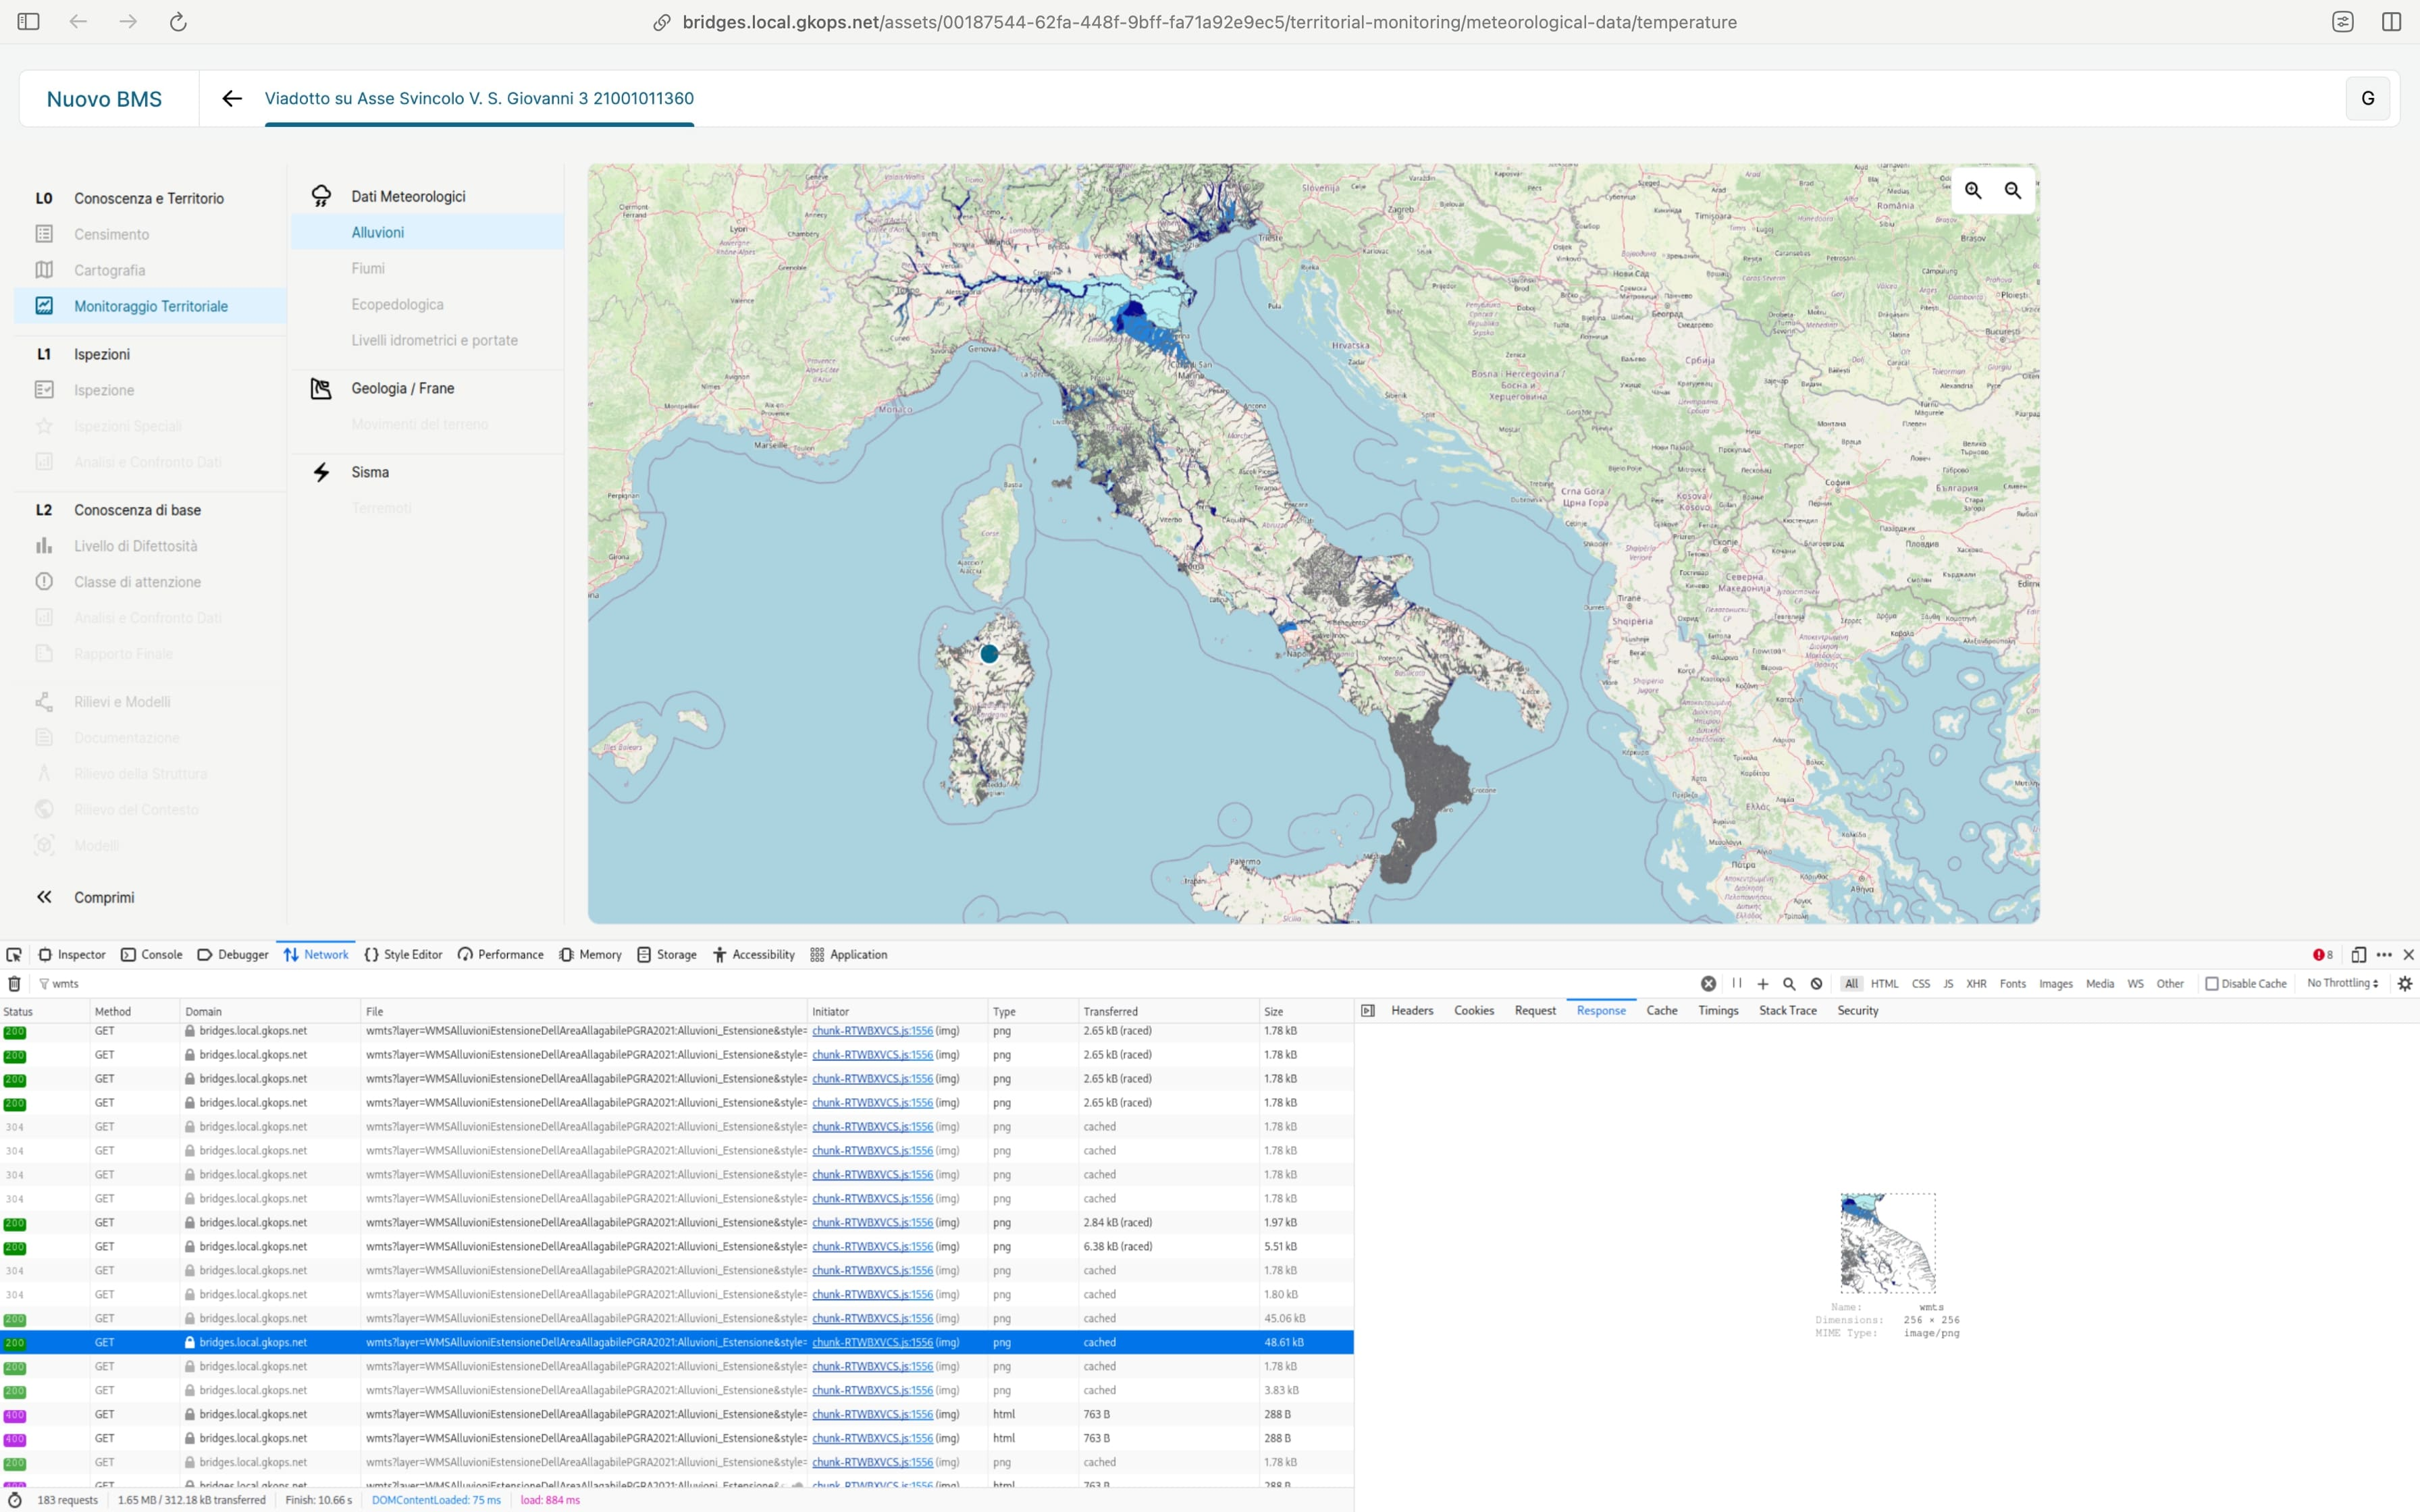
\includegraphics[width=1\textwidth]{Tesi/images/Capitolo5/italiaAlluvioniWMTS.jpg}
      \caption{Alluvioni - Estensione dell’area allagabile (PGRA 2021) - WMTS}
      \label{fig:italiaAlluvioniWMTS}
\end{figure}

\subsection{Implementazione del formato Shapefile}

Un altro formato di mappa geospaziale che doveva ancora essere implementato, era il formato shapefile, utilizzato dagli enti IdroGEO e GeoCart per fornire le loro mappe. Fino a quel momento, il formato shapefile non era stato considerato, in quanto OpenLayers non lo supporta nativamente. Di conseguenza, le mappe di GeoCart non erano ancora state integrate, mentre quelle di IdroGEO per semplicità erano state implementate soltanto in GeoJSON, dato che erano fornite anche in quel formato. 
\\Per risolvere il problema, si è inizialmente ipotizzato di passare attraverso l'uso di librerie di terze parti che consentissero la conversione del formato shapefile in un altro formato, come il GeoJSON. Tuttavia, con quel tipo di implementazione, sarebbero comunque persistite le problematiche già spiegate in precedenza, oltre al fatto che non ci sarebbe stata garanzia circa la correttezza della conversione al nuovo formato. Inoltre, considerata la mole degli shapefiles, sarebbe risultato necessario partizionare i dati e gestirne il recupero parziale.
\\Pertanto, si è pensato di appoggiarsi nuovamente al GeoServer, che supporta shapefile come formato e lo espone in vari protocolli, tra cui quelli fino ad ora implementati. Ciò ha ovviamente facilitato la parte di sviluppo, in quanto non è stato necessario programmare alcuna funzionalità per supportarlo: lato back-end, infatti, è stato sufficiente caricare il file della mappa all'interno del volume (del container Docker di GeoServer) e poi, utilizzando l'interfaccia grafica di GeoServer, renderlo disponibile come layer. Lato front-end, invece, non è stato necessario modificare alcuna classe, ed è bastato richiedere la nuova mappa al GeoServer come fatto precedentemente.
\\Per verificare il suo funzionamento è stata scelta una nuova mappa, fornita dall'ente GeoCart che rappresentava il "Reticolo Idrografico" nella regione della Calabria \ref{fig:calabriaAlluvioni}.
Per semplicità, il tirocinante ha deciso di far richiedere al client prima la mappa nel protocollo WMS, così da controllare se questa venisse rappresentata correttamente e nella giusta proiezione, e solo dopo averla verificata, farla richiedere anche in WMTS.
\\Infatti, l'unica problematica riscontrata in questa implementazione è stata che la mappa conteneva, all'interno del suo shapefile, una proiezione non nota a GeoServer, andando così a mostrare a schermo la mappa a delle coordinate sbagliate.
Per risolvere il problema, invece di utilizzare Proj4J come fatto precedentemente, è stato sufficiente, attraverso l'interfaccia grafica di GeoServer, impostare forzatamente una nuova proiezione: attivando l'impostazione "Force Declared", infatti, GeoServer si è occupato in automatico di sovrascrivere la vecchia proiezione con la nuova scelta, cercando di mantenere nel modo più fedele possibile la rappresentazione della mappa. Per limitare il rischio di errore dovuto al cambio di proiezione, è stato sufficiente cercare, con l'aiuto del tutor aziendale, una nuova proiezione che fosse compatibile con quella utilizzata all'interno dello shapefile, riuscendo così a mostrare correttamente la mappa a schermo. 
\\Inoltre, questa soluzione ha anche diminuito il carico di lavoro lato front-end, avendo spostato il compito di registrare ed eseguire il cambio di proiezione su GeoServer. Ovviamente, avendo caricato la mappa direttamente all'interno di GeoServer, senza dover passare da un server esterno come negli altri casi, la sua visualizzazione è stata pressoché immediata.
\begin{figure}[htbp]
      \centering
      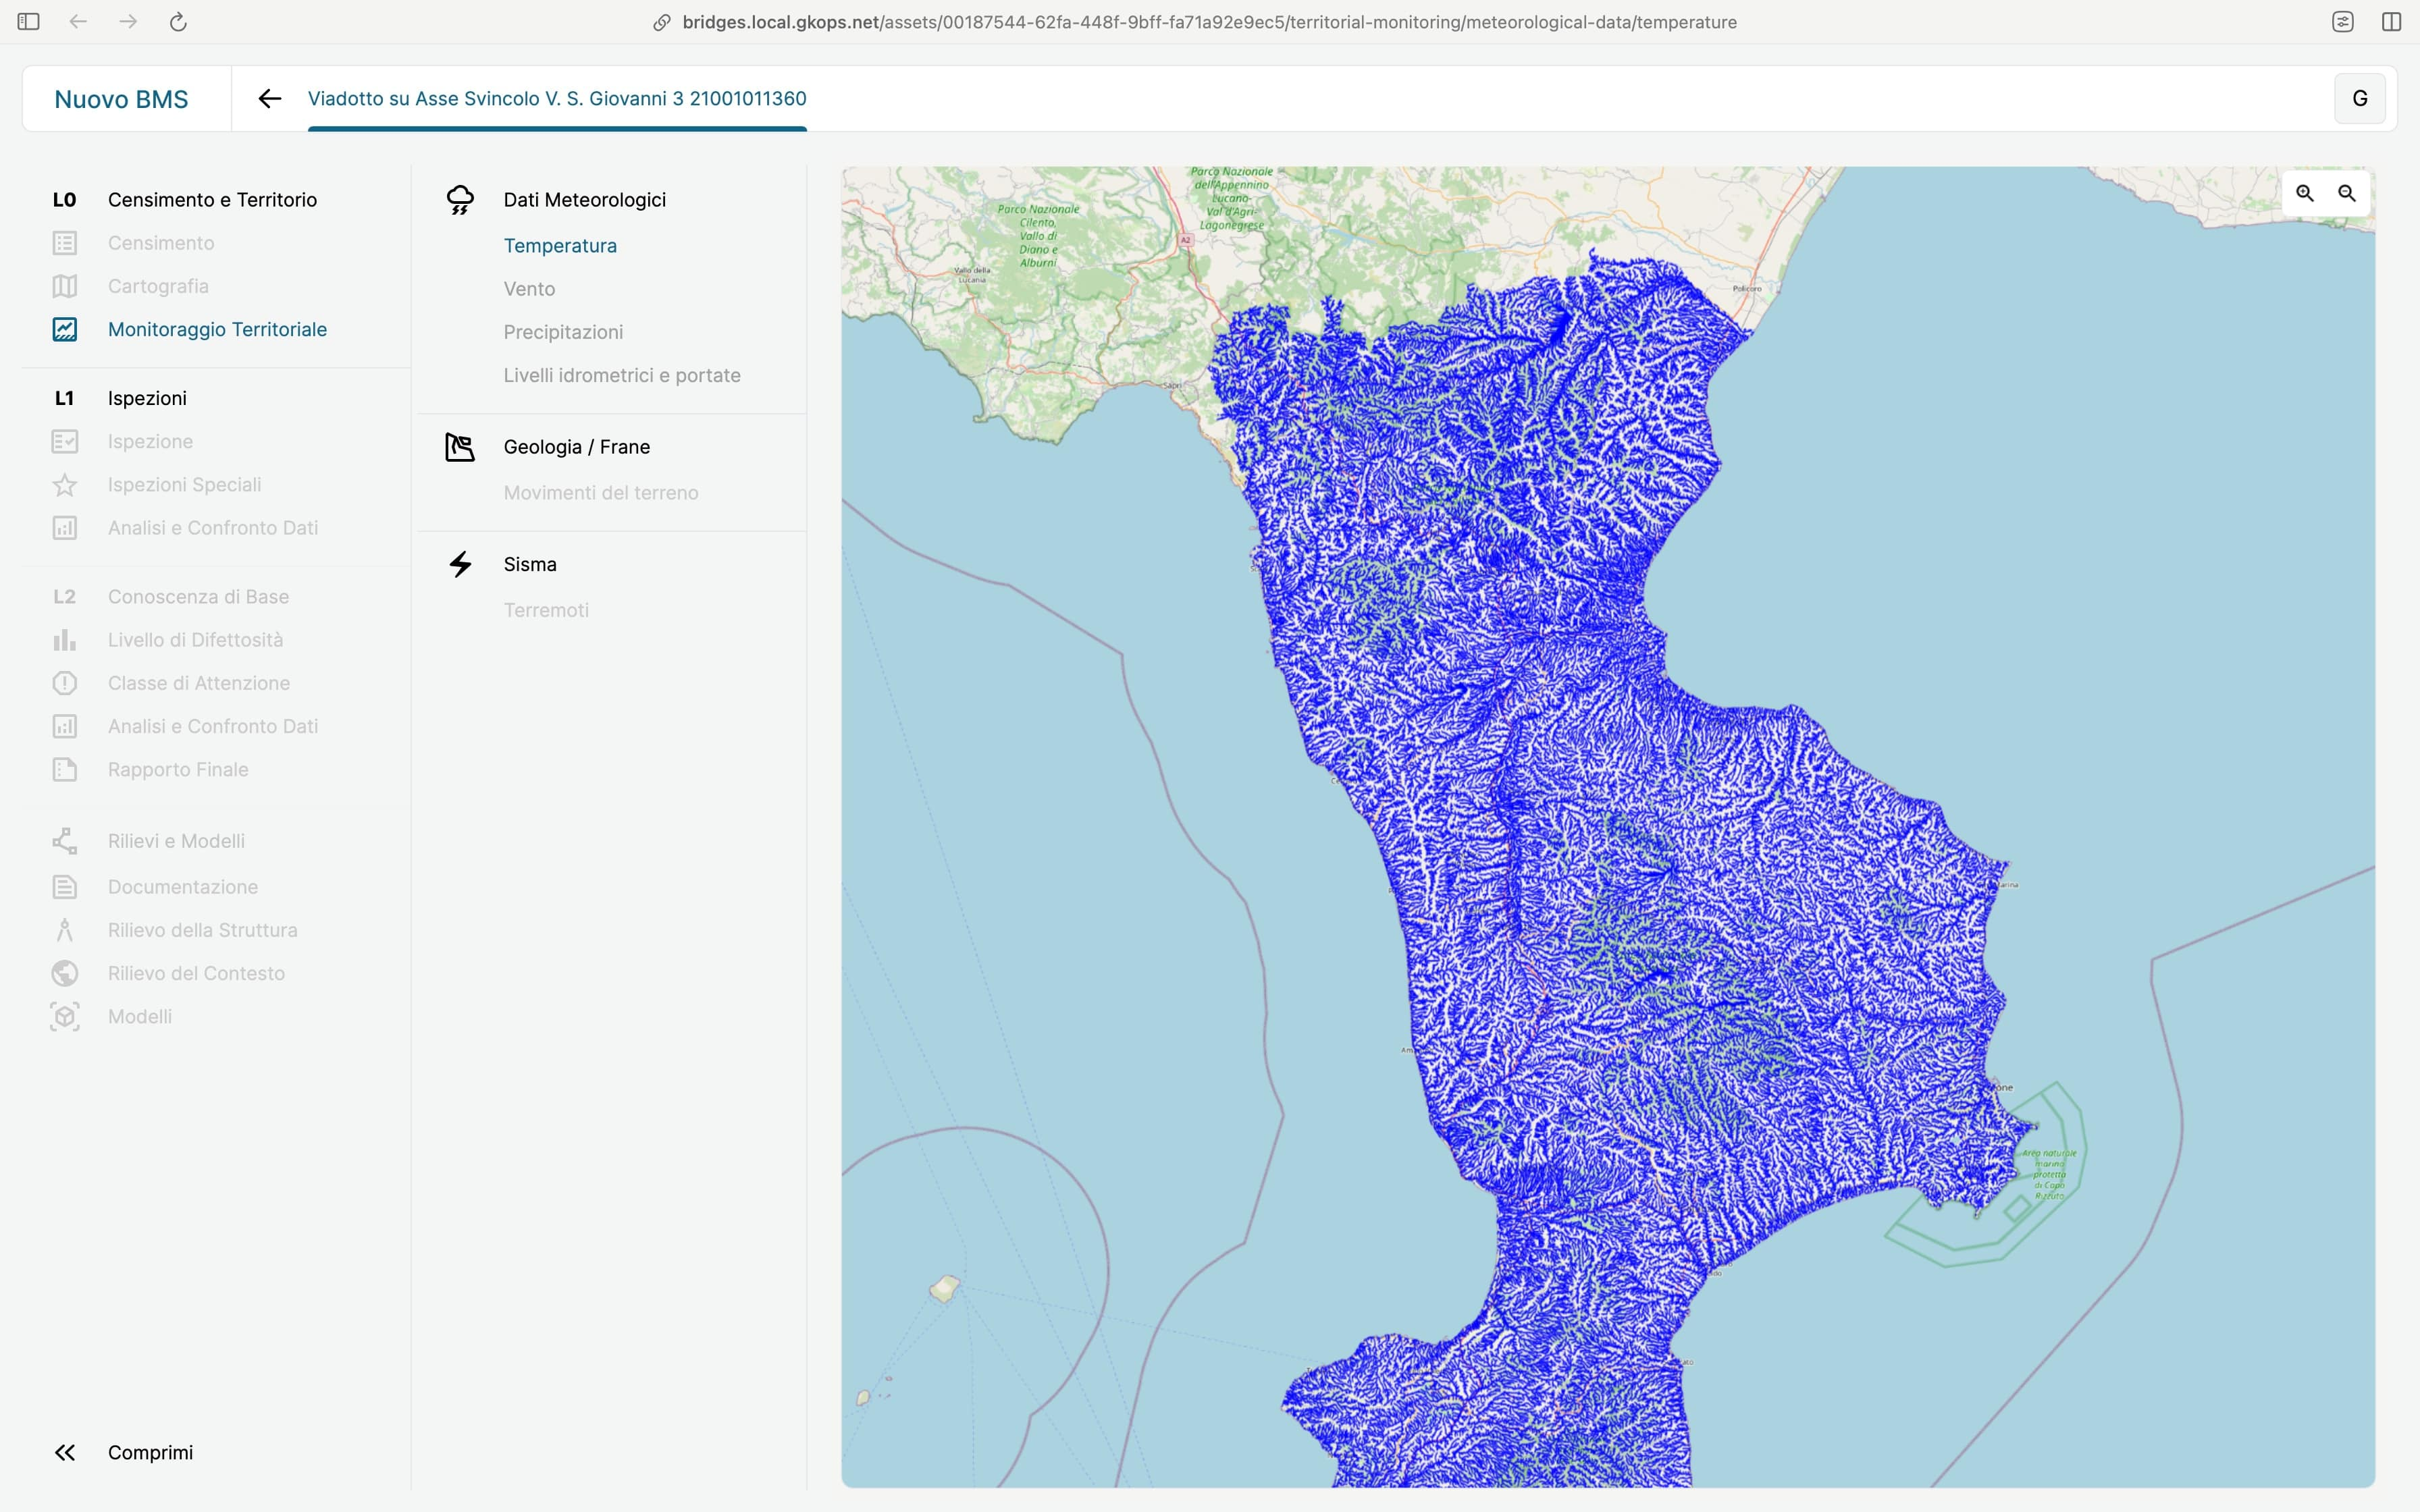
\includegraphics[width=1\textwidth]{Tesi/images/Capitolo5/calabriaAlluvioni.jpg}
      \caption{Calabria Reticolo Idrografico - WMTS}
      \label{fig:calabriaAlluvioni}
\end{figure}
\newpage
\subsection{Implementazione del formato SLD}

Alcune delle mappe fornite da questo ente, oltre al formato shapefile, comprendevano dei file aggiuntivi in formato SLD. Questi file si occupavano, similmente al ruolo del CSS nelle pagine HTML, di definire uno stile specifico per la rappresentazione dei dati della mappa. Questi file, inoltre, potevano contenere al loro interno l'immagine di una legenda, la quale serviva per rappresentare il motivo dello stile applicato alla mappa (generalmente, questo tipo di immagine è quello che viene restituito come risposta alla richiesta di GetLegendGraphic, nel protocollo WMS).
\\Il tirocinante si è quindi occupato di integrare all'interno del progetto le mappe con questo stile, sfruttando anche in questo caso le funzionalità offerte da GeoServer.
\\Il lavoro è cominciato inserendo al suo interno una delle mappe in formato shapefile, privandola del suo file di stile, in modo da osservare le differenze della mappa con e senza quest'ultimo applicato; oltre che verificare la posizione corretta della mappa. Questa, nota con il nome di "EGMS Calabria", è stata richiesta dal client sia tramite protocollo WMS che WMTS (utilizzando la stessa implementazione fatta precedentemente), riuscendo così in entrambi i casi a visualizzarla correttamente. Tuttavia, in maniera conforme alle previsioni, lo stile della mappa applicato non era quello corretto, e di conseguenza, la mappa veniva mostrata con lo stile di base fornito da GeoServer. Nell'immagine \ref{fig:calabriaNoSLD} viene mostrata la mappa con lo stile di default applicato da GeoServer.
\\~\\ %<- fixme
\begin{figure}[htbp]
      \centering
      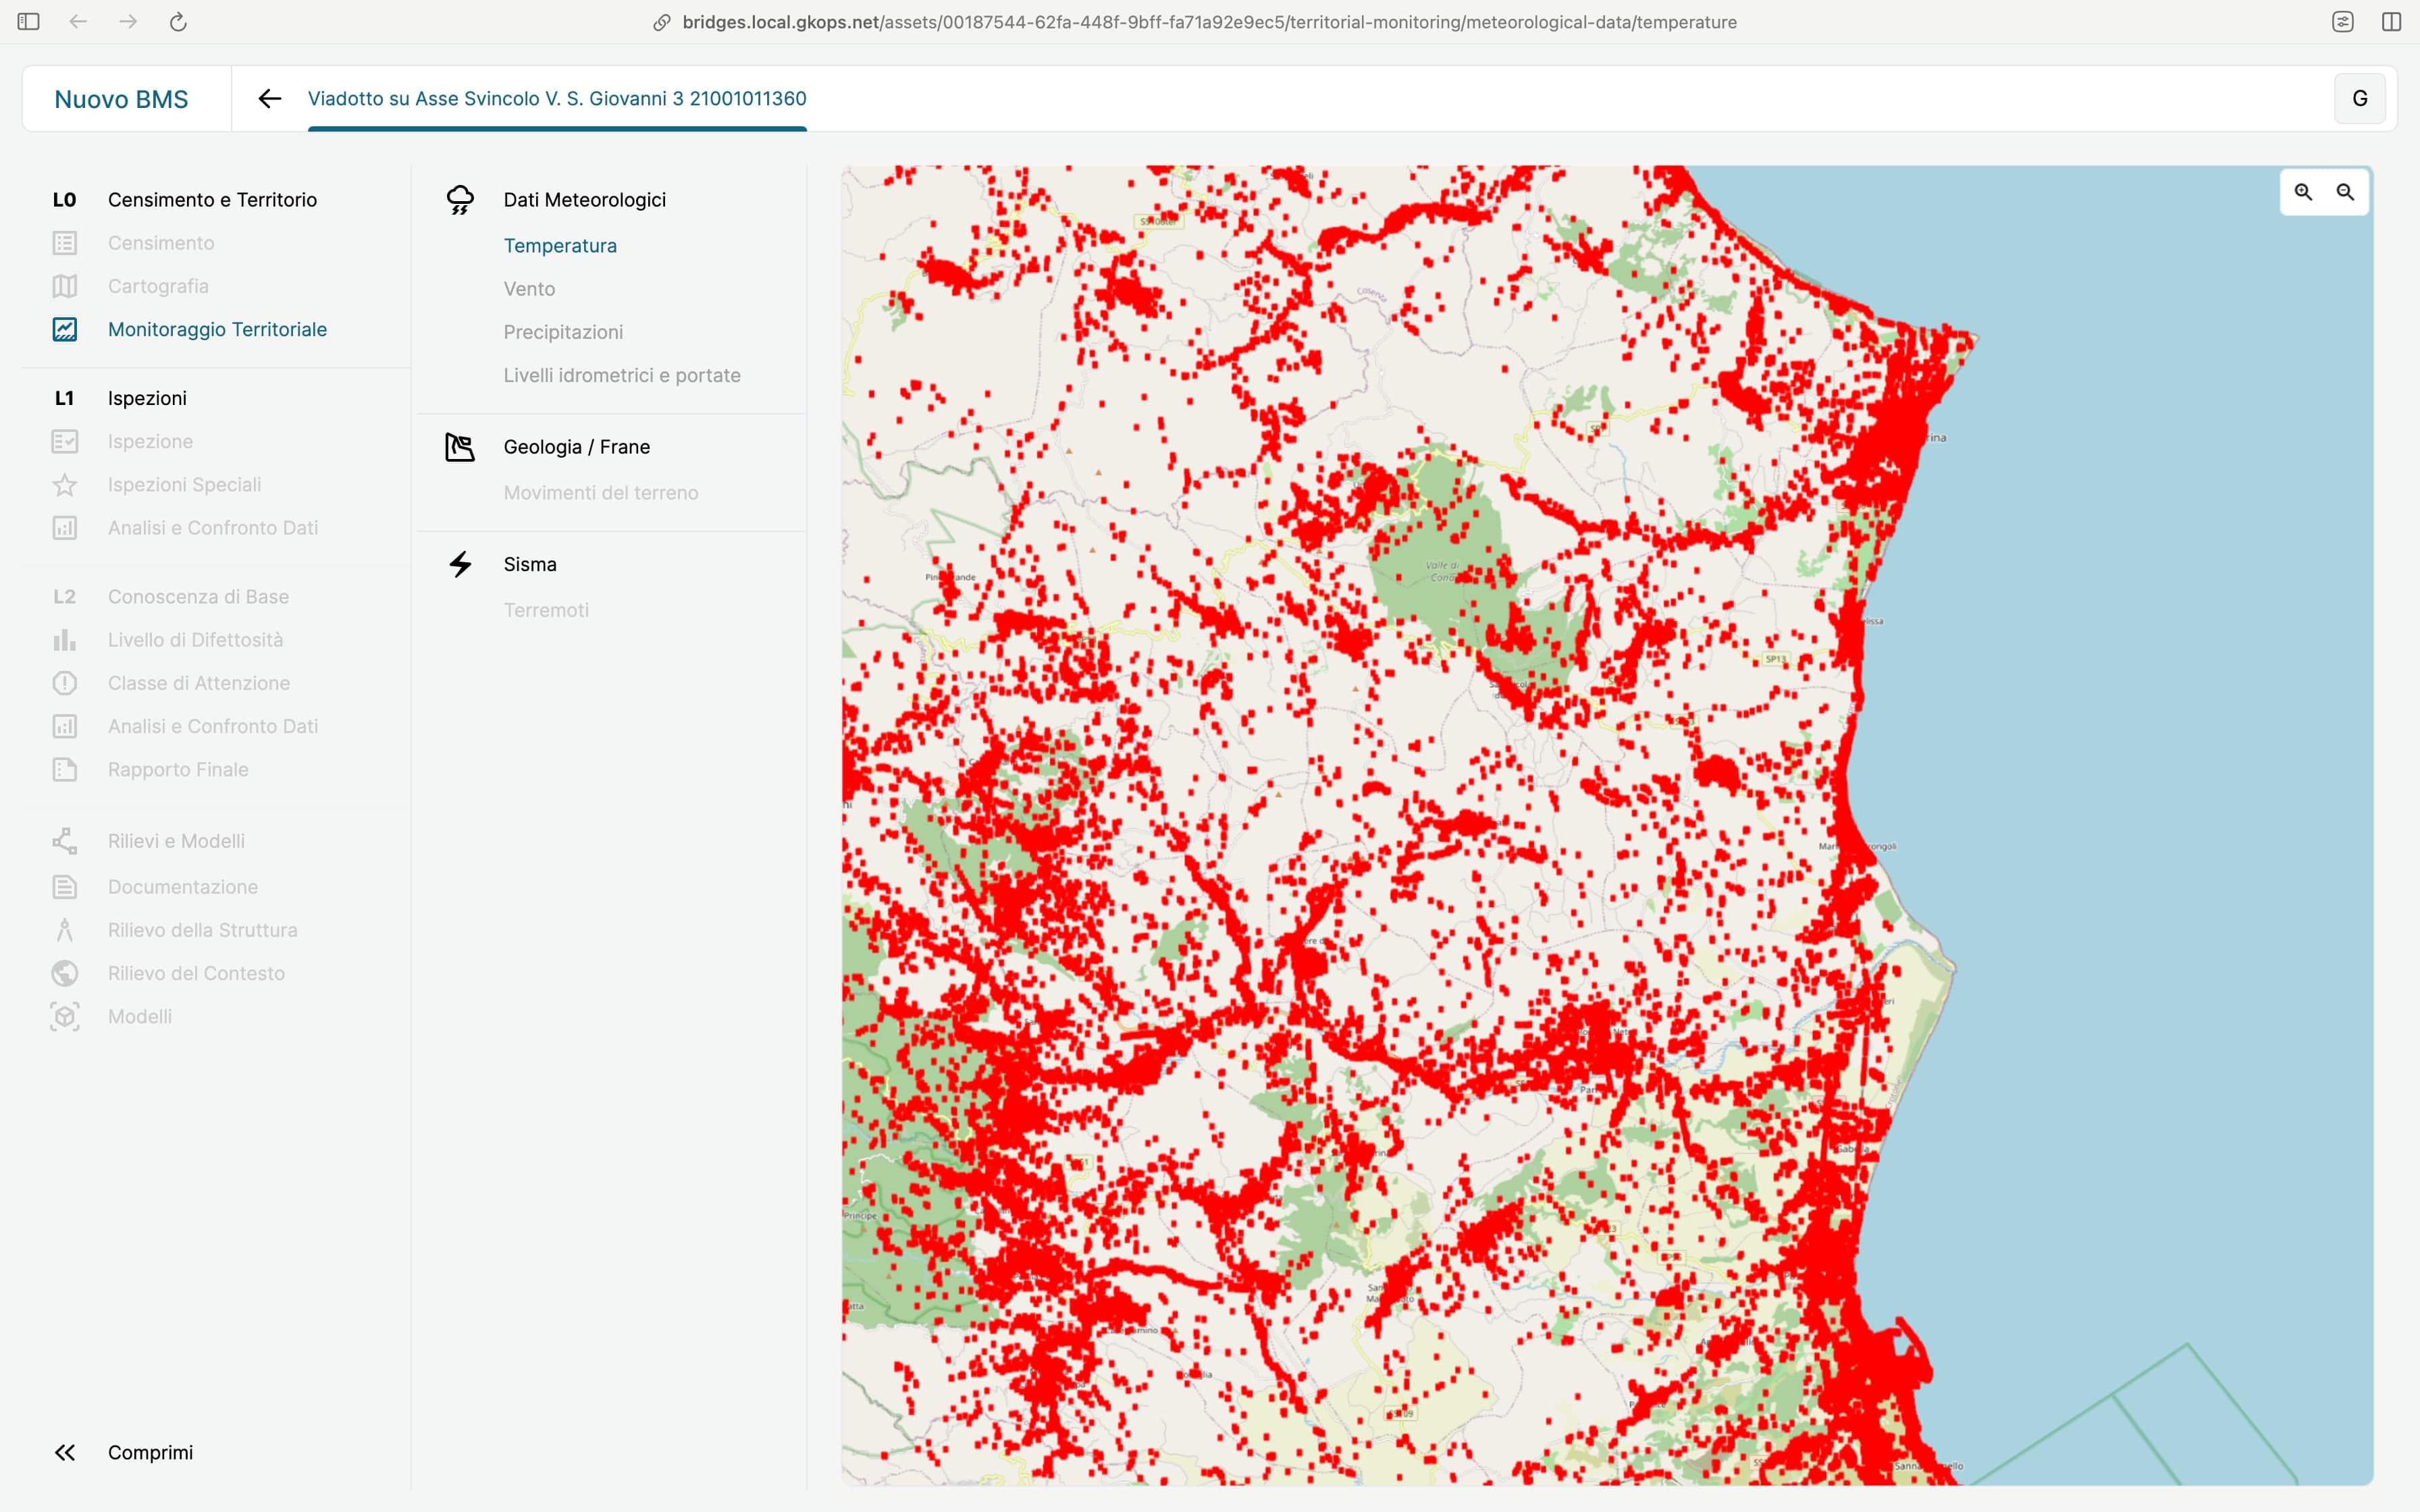
\includegraphics[width=1\textwidth]{Tesi/images/Capitolo5/calabriaNoSLD.jpg}
      \caption{EGMS Calabria - priva di stile SLD}
      \label{fig:calabriaNoSLD}
\end{figure}
\\Per applicare lo stile allo shapefile è stato prima caricato un nuovo file SLD (attraverso l'interfaccia grafica di GeoServer), seguendo una procedura simile a quella adottata per caricare una mappa e poi, è stato sufficiente selezionare la mappa su cui applicare lo stile. GeoServer offriva sia la possibilità di sovrascrivere lo stile corrente, applicando così quello appena caricato, sia di avere molteplici stili disponibili, in modo che il client potesse richiederne uno fra questi. Poiché erano presenti delle mappe che potevano essere visualizzate con più stili differenti, come ad esempio, la mappa scelta che aveva due file SLD chiamati "L2b Generale" e "L2b Dettagliato", si è scelto di non sovrascrivere lo stile ma di mantenerne molteplici.
\\Lato front-end, è stato quindi necessario modificare il codice affinché si riuscisse, oltre che a visualizzare la mappa, a richiedere al server quali fossero gli stili disponibili per quest'ultima. Queste informazioni, insieme a quelle riguardanti il layer (tipo di proiezioni, formato, etc...), erano ottenibili tramite la richiesta di GetCapabilities.
\\Quindi, il codice per recuperare la mappa mediante protocollo WMTS è stato ulteriormente modificato affinché, mediante \verb|WMTSCapabilities|, si riuscisse a estrapolare, oltre che al nome del layer e la rispettiva proiezione, anche l'elenco di tutti gli stili disponibili. Una volta ottenuto, è stato sufficiente passare come argomento alla classe \verb|WMTS| anche il nome dello stile da visualizzare.
\medskip
\\L'ultimo compito da svolgere è stato quello di riuscire a far ottenere l'immagine della legenda al front-end, in modo da poterla visualizzare affiancata alla mappa stessa. La legenda, salvata anch'essa all'interno di GeoServer, poteva essere reperita attraverso una richiesta di GetLegendGraphic, mediante protocollo WMS. Poiché il client era già a conoscenza delle informazioni della mappa, in quanto aveva appena compiuto una richiesta di GetCapabilities tramite protocollo WMTS, non gli era necessario, per ottenere la legenda, fare di nuovo una richiesta di GetCapabilities tramite protocollo WMS, ma gli era sufficiente richiedere direttamente l'immagine della legenda con la richiesta GetLegendGraphic.
\\Il codice è stato quindi nuovamente modificato, facendo in modo che, a seguito della visualizzazione della mappa, il front-end effettuasse una nuova richiesta HTTP al GeoServer, così da recuperare direttamente l'immagine della mappa. Nell'immagine \ref{fig:calabriaSLDLegenda} è mostrata la mappa con lo stile SLD applicato, accompagnata dalla relativa legenda.
\begin{figure}[htbp]
      \centering
      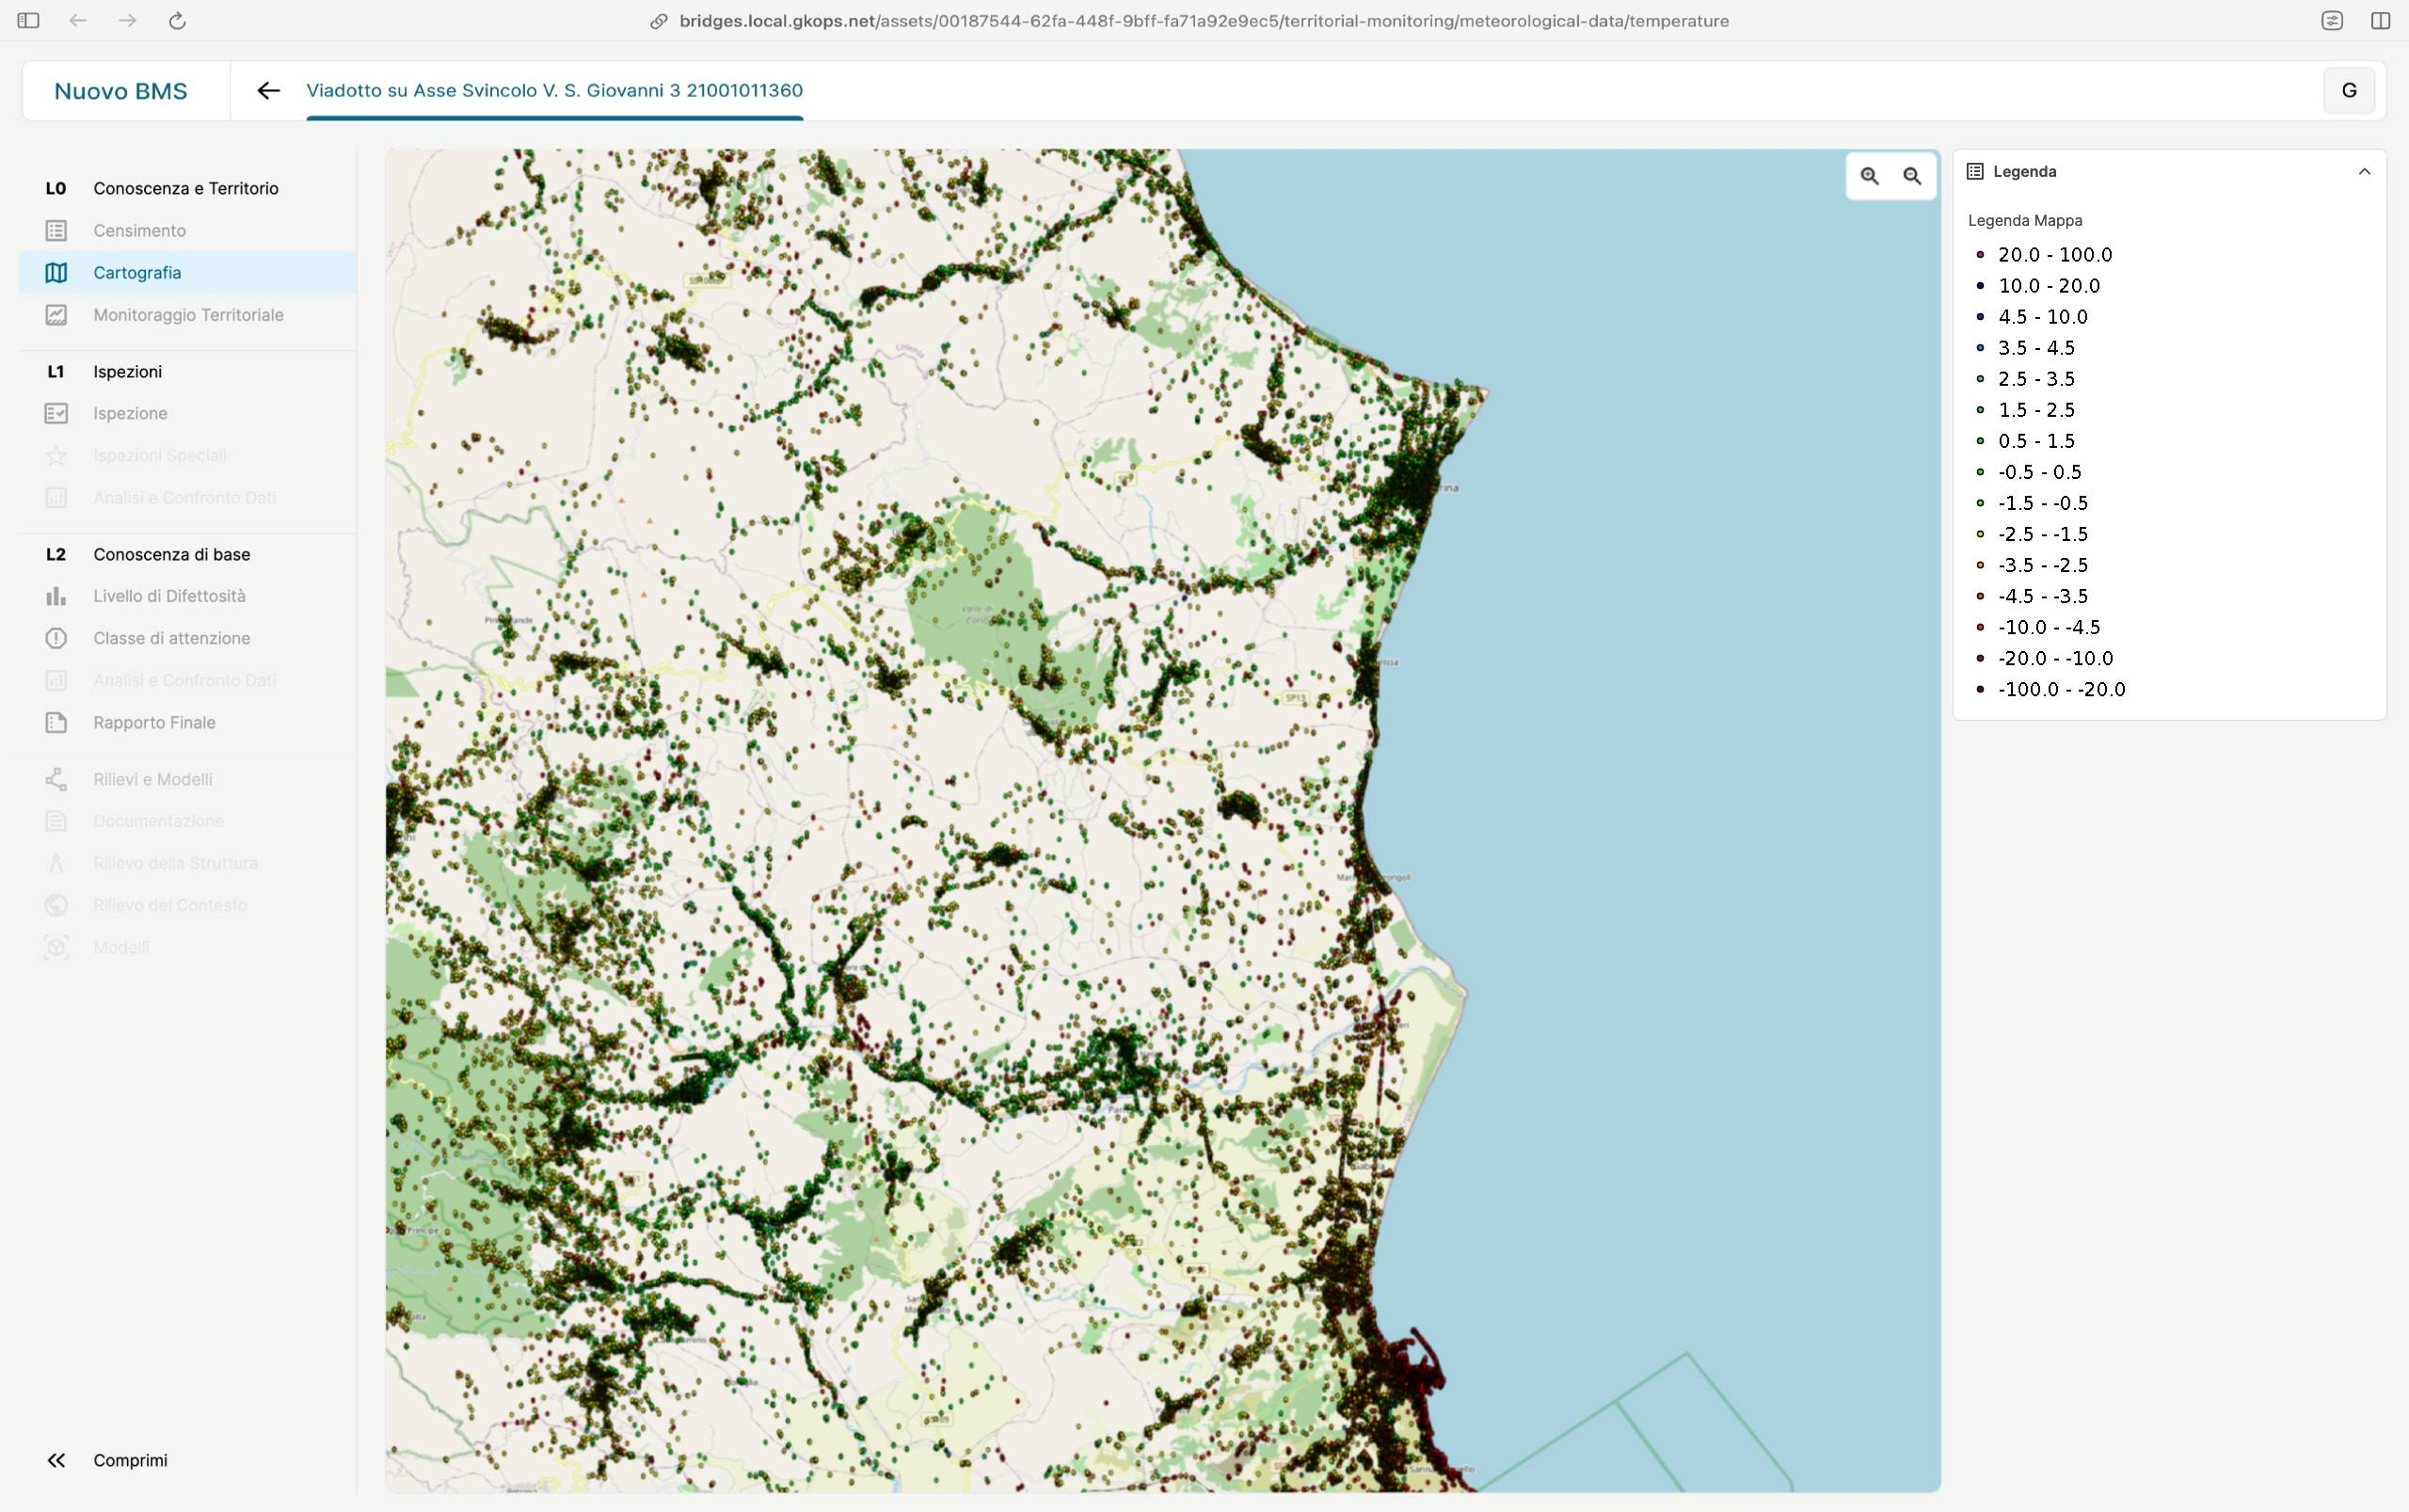
\includegraphics[width=1\textwidth]{Tesi/images/Capitolo5/calabriaSLDLegenda.jpg}
      \caption{EGMS Calabria - con stile SLD applicato}
      \label{fig:calabriaSLDLegenda}
\end{figure}

\subsection{Implementazione protocollo WFS}

L'ultima implementazione rimasta da fare era quella del protocollo WFS. Per renderlo supportato dal front-end, è stato sufficiente sviluppare un codice simile a quello utilizzato precedentemente per il formato GeoJSON, con l'unica differenza di contattare direttamente il GeoServer, invece di recuperare i dati della mappa dal file locale salvato nel progetto. Il GeoServer, infatti, offriva la possibilità di fornire i dati delle mappe anche in questo formato (per il protocollo WFS), evitando così di dover scrivere ulteriore codice per supportarne uno nuovo.
\\In maniera analoga alle altre implementazioni, il candidato ha innanzitutto modificato le classi \verb|BuildLayer| e \verb|MapModel|, aggiungendo come nuovo tipo il WFS. Successivamente, come fatto per il GeoJSON, ha di nuovo utilizzato la stessa classe (chiamata anch'essa \verb|GeoJSON|) fornita dalla libreria OpenLayers stessa. A quest'ultima ha infine passato come argomento l'url della mappa da reperire, invece del percorso locale all'interno del progetto. Precisamente, l'url corrispondeva ad una richiesta di GetFeature al GeoServer, richiedendo tramite query parameters: il formato della mappa (richiesto appunto in JSON), il nome della mappa, la proiezione e infine un parametro che permetteva di limitare il numero di feature da farsi restituire dal server. Infatti, a differenza della vecchia implementazione, il GeoServer (mediante protocollo WFS) permetteva di effettuare delle manipolazioni sulle feature, prima che queste venissero effettivamente restituite. Da quel momento, è stato quindi possibile far richiedere dal client, se necessario, una serie di parametri aggiuntivi all'interno della richiesta che permettessero operazioni come l'ordinamento, il filtraggio, etc...
\\Tali operazioni potevano essere svolte anche unicamente lato front-end, ma come già spiegato, ciò avrebbe richiesto un dispendio elevato di risorse, in quanto tutte le feature sarebbero dovute essere tenute in memoria.